\documentclass[11pt]{amsart}


\usepackage{geometry}                % See geometry.pdf to learn the layout options. There are lots.
\geometry{a4paper}                   % ... or a4paper or a5paper or ...
%\geometry{landscape}                % Activate for for rotated page geometry
\usepackage[parfill]{parskip}    % Activate to begin paragraphs with an empty line rather than an indent
\usepackage{enumitem}
\usepackage{graphicx}
\usepackage{amssymb}
\usepackage{amsmath}
\usepackage{cancel}
\usepackage{tikz}
\usepackage{epstopdf}
\DeclareGraphicsRule{.tif}{png}{.png}{`convert #1 `dirname #1`/`basename #1 .tif`.png}
\usepackage{breqn}

\usetikzlibrary{calc,intersections,through,backgrounds,arrows,decorations.markings}

\tikzset{
  coordsys/.pic={
    \draw[->] (0,0) -- ++(6mm,0pt);
    \draw[->] (0,0) -- ++(0pt,6mm);
  },
  myarr/.style={decoration={
      markings,
      mark=between positions 0 and 1 step 2mm with {\arrow{stealth}},
    },
    postaction=decorate
  },
}

\title{Econ 210C Problem Set \# 2}
\author{Nathaniel Bechhofer}
%\date{}                                           % Activate to display a given date or no date

\begin{document}




\maketitle

\section{Investment and the Housing Market}

\subsection*{(a)}
\begin{enumerate}
	\item $I = \psi (P)$: Gross investment in housing is an increasing function of the price of houses. This specification implies that housing investment can be interpreted as the supply of new housing. 
	\item $r + \delta = (R + \dot{P})/P$: This implies that the costs of investing into a house, namely forgone investment income and depreciation are equal to the benefits, namely rental payments and capital gains. 
	\item $R = R(H)$: Rental cost is a decreasing function of the size of the housing stock. 
	\item $\dot{H} = I - \delta H$: The housing stock can change in two ways, housing investment and depreciation.
\end{enumerate}

\subsection*{(b)}

We merely substitute to obtain

\begin{align*}
\dot{H} &= \psi(P) - \delta H \\
r + \delta &= (R(H) + \dot{P}) / P
\end{align*}




\begin{figure}[htbp]
\begin{center}
\begin{tikzpicture}[x=3cm,y=3cm]
\draw [name path=A--B]
(0.2,0.5) -- 
(1.8,1.5) node[right] {$\dot{H} = 0$};
\draw[name path=C--D]
(0.2,1.5) to[bend right] 
(1.8,0.5) node[right] {$\dot{P} = 0$};
\path [name intersections={of=A--B and C--D,by=E}];
\node [fill=red,inner sep=1pt] at (E) {};
\draw[->]
  (-0.1,0) -- (2,0) node[right] {$H$};
\draw[->]
  (0,-0.1) -- (0,2) node[above] {$P$};
\draw[myarr]
  (0.2,1) -- 
  (E);
\draw[myarr]
  (1.6,0.8) -- 
  (E);
\path
  pic[yscale=-1] at (0.3,1) {coordsys}
  pic[xscale=-1] at (1.7,1) {coordsys}
  pic at (0.8,1.7) {coordsys}
  pic[rotate=180] at (1.5,0.3) {coordsys};
\end{tikzpicture}
\caption{Phase diagram for 1c}
\label{1c}
\end{center}
\end{figure}

\subsection*{(d)}

Rewriting the equation for $\dot{P}$ gives 
\[
\dot{P} + R(H) = P (r + \delta)
\]
implying an increase in $r$ must increase $R(H)$ correspondingly given $\dot{P} = 0$. 
Since $R$ is a decreasing function of $H$, we have that $H$ decreases and the $\dot{P} = 0$ locus shifts to the left.

\subsection*{(e)}

If we go from $r$ to $r^{*}$, where $r < r^{*}$, then $P$ immediately drops to the level $\frac{R(H)}{r^{*} + \delta}$, as the higher opportunity cost of investing in housing reduces the quantity of housing investment.
As housing investment decreases, the quantity of housing stock decreases gradually until $R(H)$ goes up to the $\dot{P}=0$ point. 
So we have that $H$ moves gradually down to the new steady state, $P$ drops immediately then rises to its new but lower level, $I$ drops immediately then rises to its new lower level, and $R$ rises gradually to its new steady state level.

\begin{figure}[htbp]
\begin{center}
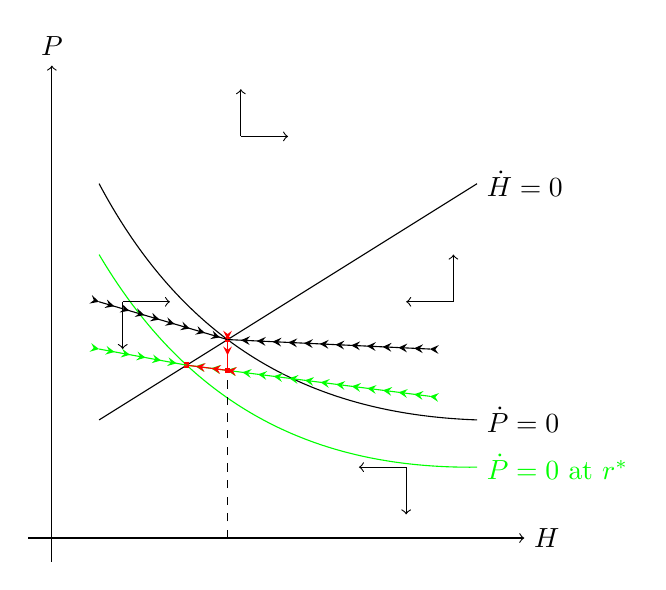
\begin{tikzpicture}[x=3cm,y=3cm]
\draw [name path=A--B]
(0.2,0.5) -- 
(1.8,1.5) node[right] {$\dot{H} = 0$};
\draw[name path=C--D]
(0.2,1.5) to[bend right] 
(1.8,0.5) node[right] {$\dot{P} = 0$};
\path [name intersections={of=A--B and C--D,by=E}];
\draw[name path=F--G, color=green]
(0.2,1.2) to[bend right] 
(1.8,0.3) node[right] {$\dot{P} = 0$ at $r^{*}$};
\path [name intersections={of=A--B and F--G,by=H}];
\node [fill=red,inner sep=1pt] at (E) {};
\draw[->]
  (-0.1,0) -- (2,0) node[right] {$H$};
\draw[->]
  (0,-0.1) -- (0,2) node[above] {$P$};
\draw [dashed, name path=Hdash] 
  ($(-0.1,0)!(E)!(2,0)$) -- (E);
\node [fill=red,inner sep=1pt] at (H) {};
\draw[myarr]
  (0.2,1) -- 
  (E);
\draw[myarr]
  (1.6,0.8) -- 
  (E);
\draw[myarr, color=green]
  (0.2,0.8) -- 
  (H);
\draw[myarr, color=green, name path=J--K]
  (1.6,0.6) -- 
  (H);
\path [name intersections={of=Hdash and J--K,by=J}];
\node [fill=red,inner sep=1pt] at (J) {};
\draw[myarr, color=red]
  (E) -- 
  (J);
\draw[myarr, color=red]
  (J) -- 
  (H);
\path
  pic[yscale=-1] at (0.3,1) {coordsys}
  pic[xscale=-1] at (1.7,1) {coordsys}
  pic at (0.8,1.7) {coordsys}
  pic[rotate=180] at (1.5,0.3) {coordsys};
\end{tikzpicture}
\caption{Change in the real interest rate}
\label{1e}
\end{center}
\end{figure}

\subsection*{(f)}

$P$ will still drop immediately, but to a level higher than $\frac{R(H)}{r^{*} + \delta}$, because we still have that the higher opportunity cost of investing in housing reduces the quantity of housing investment.
As housing investment decreases, the quantity of housing stock decreases at first, leveling off during the period increased interest rates, after which it rises again forever back up to the original $\dot{P}=0$ point. 
So we have that $H$ moves gradually down until it starts rising again (before the increase is over) to the same steady state, $P$ drops immediately then rises back to its original level (with a discrete jump when the increase is over), $I$ drops immediately then rises back to its original level (with a discrete jump when the increase is over), and $R$ rises gradually until it levels off at the same point $H$ does, after which it gradually falls to the same steady state level.

\subsection*{(g)}

$P$ will still drop immediately, and then gradually declines further until it hits $\frac{R(H)}{r^{*} + \delta}$ (with a discrete drop when the increase hits).

$H$ declines gradually starting immediately toward the new lower steady state value. 

$I$ drops immediately, then rises to its new lower level.

$R$ increases gradually starting immediately toward the new higher steady state value.


\subsection*{(h)}

In this case, we merely have
\[
r + \delta = R(H) / P
\]
so an increase in $r$ implies an immediate fall in $P$

$P$ will drop immediately, and then rises slowly to its new steady state value. 

$H$ declines gradually; $(H,P)$ moves along the $\dot{P} = 0$ locus.

$I$ drops immediately, then rises to its new lower level.

$R$ increases gradually starting immediately toward the new higher steady state value.

\subsection*{(i)}

If people have static expectations and there is an interest rate shock, then the model matches everything in the housing crisis; prices and construction dropped rapidly, while there was little effect on rental costs.



\end{document}

